\section{Control}
Control is an essential aspect of any generative model. Without control, even the best generative models producing beautiful music would be of very limited real-world use. Control allows generative AI tools to become proper collaborative systems, and generate for a wide array of scenarios. In music generation control covers essentially all musical parameters. Parameters vary by representation, symbolic music for instance leaves very little room for any type of timbre control (aside from instrument selection). “Raw” audio models such as Stable Audio (Evans et al., 2024) can for instance be controlled for acoustic settings (i.e jazz music playing in a busy restaurant, in a \textit{large cathedral}, or \textit{through an intercom}), something that is simply not represented in symbolic music. For musical parameters represented in symbolic music, there are different approaches to classifying them. We can differentiate between global and local features \cite{Van_Kranenburg_Volk_Wiering_2013} or deep vs surface-level features \cite{Blacking_1971}. 

\textbf{Global features} in music generation encompass high-level descriptors such as genre, function, and instrumentation/orchestration. Global features also incorporate summarizing features, that are calculated from the music itself. As an example, McKay’s \cite{McKay_2004} general-purpose symbolic music classification system defines over 104 global features, 37 of them used for melody descriptors such as probability distributions of note durations, intervals, and pitch classes. These global features can then be used to infer other high-level descriptors such as genre if it's unknown, they can also support music retrieval systems \cite{Van_Kranenburg_Volk_Wiering_2013}.  \textbf{Local features} describe individual sequences such as melodic, rhythmic, or harmonic sections. They are more information-rich, which may explain their superior performance in music retrieval \cite{Van_Kranenburg_Volk_Wiering_2013}. 

Also relevant in the music generation context are abstract vs concrete features. Music generation can take abstract concepts such as genre \cite{Rouard_Adi_Copet_Roebel_Défossez_musicgenstyle_2024}, \cite{Lu_Xu_Kang_Yu_Xing_Tan_Bian_MuseCoco_2023} or emotion \cite{Tan_Herremans_2020} \cite{Lu_Xu_Kang_Yu_Xing_Tan_Bian_MuseCoco_2023} into account, which in turn effects more complex dynamics of concrete features. To illustrate: In Music FaderNets \cite{Tan_Herremans_2020} the authors use a variational autoencoder to disentangle the abstract concept of arousal, into several concrete features including rhythmic density, note-density, tempo and dynamic, key. This allows them to change the abstract variable arousal, which cascades into a change of underlying features. This type of disentanglement can aid in situations where labled musical data with the abstract feature is less available, it can also aid in creating more accessible and interpretable generative models.

In the context of this thesis we differentiate between global features, and fine-grained or time-varying features \cite{Rütte_figaro_2023}. What is time-varying or global is highly context dependent, a piece may have one time-signature and tempo as is assumed in \cite{Lu_Xu_Kang_Yu_Xing_Tan_Bian_MuseCoco_2023} or it may vary over time as is suggested in \cite{Rütte_figaro_2023} or \cite{Huang_Yang_remi_pop_transformer_2020}. Other time varying controls could be chords \cite{Rütte_figaro_2023}\cite{Wu_Donahue_musicontrolnet_2023}\cite{Lan_Hsiao_Cheng_Yang_musicongen_2024}\cite{Min_Jiang_Xia_Zhao_polyffusion_2023}, melody \cite{copet2023simple}\cite{Min_Jiang_Xia_Zhao_polyffusion_2023} or texture \cite{Min_Jiang_Xia_Zhao_polyffusion_2023}. For the target application in an MACT - game, time-varying controls are necessary to provide a change in music that triggers a change in the patients improvisation.
For a more complete list of the types of controls in many of the common symbolic music generators refer to table \ref{table:bigtable}
in the appendix.

\subsection{Rhythmic control}
The types of control exercised over rhythmic components varies by representation as discussed in \ref{representation}. In CocoMulla \cite{Lin_cocomulla_2024} generated audio is conditioned with drum tracks and a piano-roll. Similarly in JASCO\cite{Tal_jasco} drums are used for conditioning. In MusicConGen.\cite{Lan_Hsiao_Cheng_Yang_musicongen_2024}control for rhythm is added through tracking beats and downbeat. MusicControlNet\cite{Wu_Donahue_musicontrolnet_2023} adds beat and downbeat conditioning to an audio diffusion model.
For symbolic systems control of tempo and meter is relatively common \cite{Rütte_figaro_2023}, \cite{Huang_Yang_remi_pop_transformer_2020}, \cite{Lu_Xu_Kang_Yu_Xing_Tan_Bian_MuseCoco_2023}. More fine grained control over rhythm is sometimes deployed through note-density (both vertical and horizontal)\cite{Rütte_figaro_2023},\cite{Huang_rule_diffusion_2024}.  Another option is control over texture, which merges harmonic and rhythmic elements. In Polyffusion\cite{Min_Jiang_Xia_Zhao_polyffusion_2023}, texture is encoded by a pretrained variational auto-encoder\cite{Wang_vae_chord_rhythm_2020}. Another approach \cite{Zhu_Liu_Jiang_Zheng_texture_2024} involves passing the piano-roll as factor to guide the diffusion process.

\subsection{Target Features}
In order to extend LastMinuteGig with generated music containing appropriate cues we are targeting control of rhythmic patterns. The most simple way of targeting rhythmic patterns is through note density, implemented as a bar-level instruction of how many notes the following bar should contain. A second simple target feature is note variability (unique notes per bar over number of notes per bar). Both note-density and note-variability are simple time-varying features that are easily extracted, tokenized and introduced to the algorithm.  

A potential approach, novel to music generation, would be control mechanisms using either spectral weight or inner metric weight. Here the weight profile is passed as a control mechanism either globally or on a per bar or per section level. \textit{Comment: Introducing the control at a per bar level would be a bit odd since the idea of metric weight is about extracting weights not reflected in the symbolic grid, but it is a sensible way to introduce it to the model in bite-sized chunks able to reflect local change}. Inner metric and spectral weight weight has been successfully applied to dance music classification \cite{Chew_Volk_Lee_Dance_metric_weight_2005}, meter detection \cite{Haas_Volk_2016} and music retrieval \cite{Volk_Garbers_VanKranenburg_Wiering_Grijp_Veltkamp_2009}. This suggests that it is a powerful feature for explaining various rhythmic aspects, which may make it a good guiding mechanism. 

\section{Non neural net systems}

\subsection{Why look at non-neural systems}
While neural net systems currently receive a large amount of attention, other systems are worthy of mention. A recent study \cite{Yin_Reuben_Stepney_Collins_2023} performs a comprehensive listening survey comparing different neural net and non-neural net systems. The top-performing systems a Markov Model -  MAIA Markov \cite{Collins_Laney_2017}  and a deep learning system  - MusicTransformer \cite{Huang_Vaswani_Uszkoreit_Shazeer_Simon_Hawthorne_Dai_Hoffman_Dinculescu_Eck_2018} perform similarly well in the listening study. The choice of one of the earliest transformer based music from 2018 \cite{Huang_Vaswani_Uszkoreit_Shazeer_Simon_Hawthorne_Dai_Hoffman_Dinculescu_Eck_2018} and the restiction to symbolic music, given that the study was published in 2023 raises questions as to whether their conclusion that there is no difference in performance between the two approaches still holds, given the rapid advances in the space. However, their criticism is that many deep learning (DL) music generator projects don’t look beyond DL and compare their systems based on technical metrics with no obvious impact on how human listeners perceive the systems remain solid. The comparison between neural net and non-neural net systems is worthwhile since deep learning comes with significant downsides relating to explainability and transparency, computational efficiency, as well as copyright and licensing issues regarding their enormous data needs. Additionally, there are hybrid approaches that combine rule-based and deep-learning methods. Those methods being present in research may help researchers and developers maintain a more comprehensive toolkit of techniques and paradigms. 

\subsection{The Illiac suite, introduction to non-neural music generation}

Non-neural net systems can be roughly classified as either rule-based or statistical. Both types have been part of some of the earliest attempts at music generation. The 1957 Illiac suites \cite{Funk_2018}\cite{Hiller_Isaacson_1959} hint at many paradigms in music generation for the decades to come. Hiller \& Isaacson’s first and second movements are generated through encoding rules based on the rules of the first species counterpoint originally published in Fux’s 1725 Gradus ad Parnassum\cite{Fux_1725}, which systematically encodes Palestrina’s contrapuntal technique. Some rules aim to contain the melody, i.e. limiting the range to an octave, enforcing the same start and end note, and avoiding consecutive melodic jumps. Other rules aim to constrain harmony, such as forbidding parallel octave, fifth, and fourth motion and enforcing consonant harmonies. 

\begin{figure}[H]
    \centering
    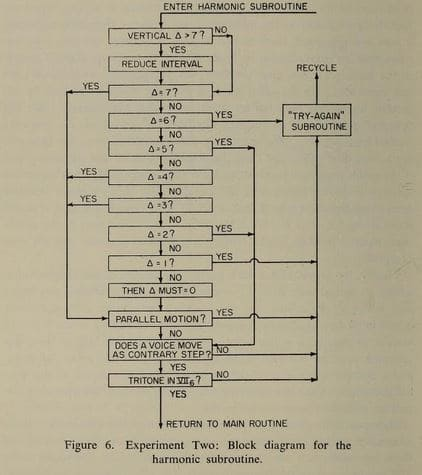
\includegraphics[width=0.5\textwidth]{IMAGES/IlliacRuleBased.jpg} 
    \caption{Rule-Based - Block Diagram from Hiller and Issacson’s book  - explaining movement two of the 1957 Illiac Suite. }
    \label{fig:hillerissacson}
\end{figure}


The third movement automates the creation of 12-tone rows, automating Arnold Schoenberg’s 12-tone technique in a semi-randomized fashion. The fourth movement involves using Markov chains with a table of possible intervals stretching from unison to octave, and probabilities assigned to each. Additional restrictions in the latter sections of the movement add memory to the method through higher-order Markov chains that reference previously generated music. 

\subsection{Rule based generation}
Centuries of style-defining musicological writing from ancient Mesopotamian tuning charts \cite{Mirelman_2013} to Fux’s Gradus ad Parnassum \cite{Fux_1725} and Arnold Schoenberg’s 12-tone music have crystallized sets of rules that approximate various styles of music. Many approaches to music generation take advantage of this knowledge and codify it into a computer program creating expert systems for music generation. This can take various forms from simple conditional state machines such as the rules in Hiller \& Isaacson’s Illiac suite with a handful of conditions to highly complex expert systems such as CHORAL \cite{Ebcioğlu_1994} (for which the developer also built a custom programming language) which encodes over 300 rules to realize bach-style chorales from a given melody.  

\subsection{Markov Model Music Generation}
Markov models remain a popular method of generating music to this day. At its simplest, a Markov music generator could work off of a transition matrix for pitch classes, such as Richard Pinkerton’s 1956 “Banal Melody Generator”\cite{Pinkerton_1956}. 
For more complex interactions, Markov chains can be nested or constrained with extensions for global structure \cite{Collins_Laney_2017}. 
Transition matrices can be built from very little data such as short improvisations used to condition the Continuator \cite{Pachet_2003}, but training over a whole corpus is also viable. 
Other systems configure Markov chains to take additional inputs into account such as Allan, \cite{Allan_2002} who generates harmonies to given melodies in the style of Bach. 

\begin{figure}[H]
    \centering
    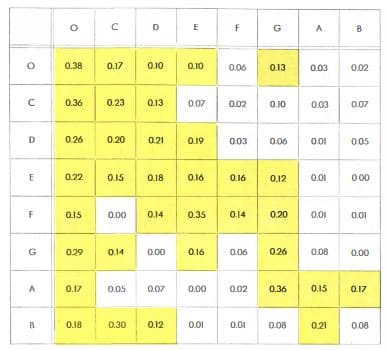
\includegraphics[width=0.5\textwidth]{IMAGES/PinkertonNurseryRhymes.jpg} 
    \caption{Transition matrix from Pinkerton's 1956 “Banal Music Generator”. Probability of a pitch (row) following on a pitch (column), likely pairs are marked in yellow. The probabilities are calculated from a set of 39 nursery rhymes.}
    \label{fig:pinkertonmatrix}
\end{figure}

\subsection{Other non-neural music generation}
Music generation has also been attempted with other means, such as metaheuristic search for harmony or melody. \cite{Altay_Alatas_2018}, evolutionary and genetic algorithms\cite{Polito_Daida_Bersano-Begey_1997}. 


\subsection{Early Neural Net based systems (up until 2018)}

Music generators based on neural nets were introduced as early as 1989. Todd et al. \cite{Todd_1989} use both a fixed window for a conventional feed-forward neural network but also introduces a feedback loop feeding the network's previous state to the next iteration, foreshadowing future work using RNNs such as \cite{Mozer_1994}. There are also hybrid systems such as HARMONET \cite{Hild_Feulner_Menzel_1991} which merge neural networks with symbolic rule-checking algorithms. More recent RNN based music generators such as FolkRNN \cite{Sturm_Ben-Tal_2016} use long short term memory (LSTM’)s or gated recurrent units (GRU’s). Generative Advesarial Networks (GANs) and Variational Autoencoders (VAEs) were and still are popular architectures for music generation. \cite{Civit_Civit-Masot_Cuadrado_Escalona_2022}

\section{State of the art - deep learning for music generation}
State-of-the-art music generation, including many commercial applications, leverages the advances in language and image generation achieved in the last five years. Two distinct approaches, namely autoregressive and diffusion-based approaches dominate.

\subsection{Transformers - sequence modelling without recurrence}
Autoregressive music generation is inspired by successful natural language modeling tasks powered by the transformer model. Transformers were originally developed for the task of language translation.\cite{Vaswani_Shazeer_Parmar_Uszkoreit_Jones_Gomez_Kaiser_Polosukhin_2017} They keep the self-attention mechanism which was deployed prior in LSTMs for seq2seq tasks \cite{Sutskever_Vinyals_Le_2014} but replace the recurrent connection with positional embeddings and masked attention. This allows the model to train on all tokens in parallel as opposed to one token at a time. At each layer a token is contextialized with the other tokens, via a paralell multi-head attention mechanism the signal of relevant tokens is enhanced, while the signal of other tokens is diminished. The transformer comes in several different configurations. The original transformer contains both encoder and decoder layers - see figure \ref{fig:transformer}. Often tasks relating to sequence understanding such as music classification use a encoder only architecture. The BERT series of language models \cite{Devlin_Chang_Lee_ToutanovaBERT_2019} and music understanding models such as MusicBERT\cite{Zeng_Tan_Wang_MUSICBERT_2021} are examples. On the other hand sequence generation tasks often employ a decoder only architecturs, this includes the GPT-series \cite{Radford_Wu_Child_Luan_gpt2_2019} and many music generators such as MusicGen\cite{copet2023simple}. The transformer architecture is the baseline for all large language models currently in use but has also been applied to modalities beyond text including images (they often form the backbone diffusion models).

\begin{figure}[H]
    \centering
    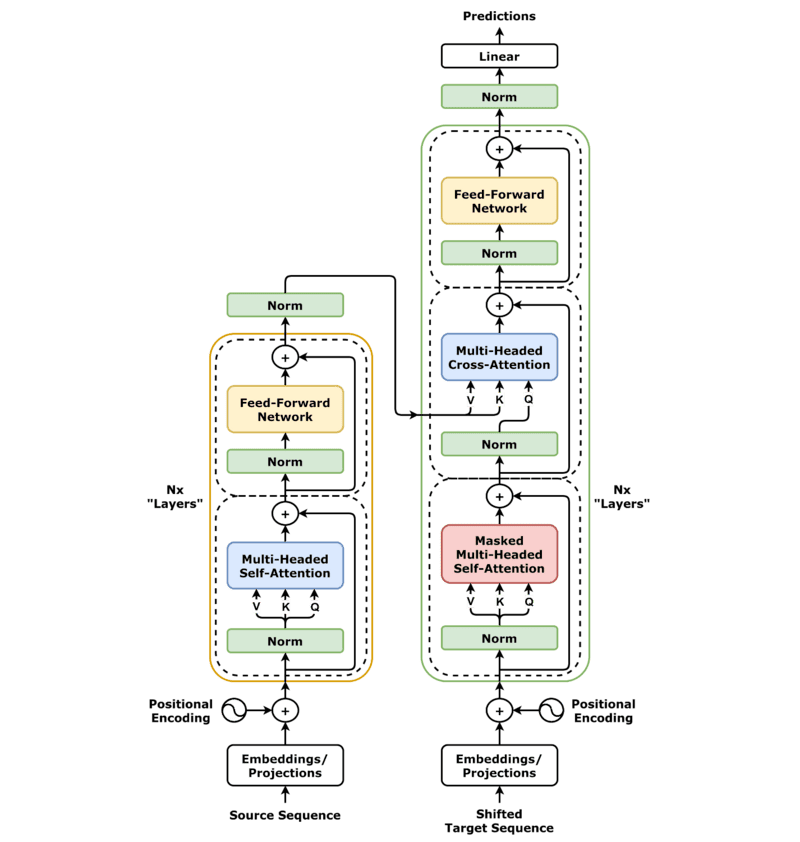
\includegraphics[width=0.5\textwidth]{IMAGES/Transformer,_full_architecture.png} 
    \caption{Schema of the full transformer encoder-decoder architecture}
    \small\textsuperscript{a=} By dvgodoy - CC BY 4.0, https://commons.wikimedia.org/w/index.php?curid=151216016
    \label{fig:transformer}
    
\end{figure}


\subsection{Diffusion models - spectrograms and piano-rolls}
Diffusion models are widely used for image and audio generation. Diffusion models learn to remove noise from a distribution (i.e an image). Random noise is added to an image, and the model learns to undo this addition. During inference the model starts with random noise (often accompanied by a guiding text prompt) and undoes it until it arrives at a clear image. AudioLDM \cite{Liu_Chen_Yuan_Mei_Liu_Mandic_Wang_Plumbley_2023}, and StableAudio \cite{Evans_Parker_Carr_Zukowski_Taylor_Pons_2024} are diffusion models that operate based on continuous audio encoding by a variational autoencoder. Diffusion models have also been used to generate symbolic music. Polyffusion \cite{Min_Jiang_Xia_Zhao_polyffusion_2023} uses image representations of piano rolls and adapt their diffusion model for various tasks, inpainting, accompaniment and melody generation and generation based on a given chord sequence or texture. 

In this thesis we will be targeting transformer models. Transformer models are tremendously popular and behind many of the state of the art results in music generation. There is a tremendous amount of interest in fine-tuning the models, and many methods developed to do so efficiently, including methods to add control. There is a fairly large selection of open-source models that generate music and very good infrastructure to support training and evaluation of those models. 

\section{Implementation of control} 
Adding control to generative models can be split into three approaches. 1: Choice of architecture and training data, 2: fine-tuning approaches, and 3: external conditioning or guidance.

\subsection{Control through architecture}
The choice of architecture lends itself to different types of control. Transformers are next token predictors, that predict based on the prior sequence. The default training paradigm allows for conditioning with a user defined musical (or audio) sequence. This is true for both audio based models such as MusicGen \cite{copet2023simple}, Jukebox \cite{Dhariwal_Jun_Payne_Kim_Radford_Sutskever_2020} and MusicLM \cite{Agostinelli_Denk_Borsos_Engel_Verzetti_Caillon_Huang_Jansen_Roberts_Tagliasacchi_et_al._2023} as well as symbolic music models such as MMT \cite{Dong_Chen_MMT_Kirkpatrick_2023}, MusicTransformer \cite{Huang_Vaswani_Uszkoreit_Shazeer_Simon_Hawthorne_Dai_Hoffman_Dinculescu_Eck_2018} and MusicBERT \cite{Zeng_Tan_Wang_MUSICBERT_2021}. 

Diffusion models are quite flexible compared to transformers, the same model can be used for inpainting, continuation and depending on the representation melody and accompaniment generation through masking.\cite{Min_Jiang_Xia_Zhao_polyffusion_2023}\cite{Rombach_Blattmann_Lorenz_Esser_Ommer_2022}

\subsection{Control through training conditioning}
Control can be added through training data. MusicGen\cite{copet2023simple}, a recent text-to-music (audio) transformer is trained on 20000 hours of licensed music from shutterstock and pond5 \footnote{https://www.shutterstock.com/music and https://www.pond5.com/} which includes textual descriptions and tags for genre, tempo, and other factors such as instrumentation. Control is achieved through the joint training of a text description and music. An example description is provided below: 

\textit{Inspirational dramatic background music! Perfect for trailer, background, advertising, historical film, movie about superheroes, teaser and many other projects!}\footnote{ https://www.pond5.com/royalty-free-music/item/95908062-inspiring-dramatic-epic-background-cinematic-music
}

Text-based control, while user-friendly and accessible to non-musicians, is inherently vague. Levels of detail and choice of words vary widely by dataset, even with standardized tags such as genre and tempo. Specialized datasets such as MusicCaps \cite{Agostinelli_Denk_Borsos_Engel_Verzetti_Caillon_Huang_Jansen_Roberts_Tagliasacchi_et_al._2023}, which contains 5500 text music pairs, with 10 seconds of music alongside a free text description and a list of aspect tags created by human experts still suffer substantially from subjectivity \cite{Lee_Doh_Jeong_2023_subjectivity_musiccaps}. 

For this reason, the creators of MusicGen \cite{copet2023simple} add melody conditioning alongside text conditioning and train their model jointly with the chromagram of the melody alongside the text.

In MusicGenStyle \cite{Rouard_Adi_Copet_Roebel_Défossez_musicgenstyle_2024} perform classifier-free guidance to add style conditioning to MusicGen. They train a music-style encoder that transforms a random subsample of a given reference audio track into tokens that are combined with the embeddings of the text-description. Both the style tokens and text tokens are provided as prefix to the model. The conditioner and the MusicGen transformer are trained jointly on the entire dataset. 

The creators of FIGARO\cite{Rütte_figaro_2023} enable fine grained control over instrumentation, note density, average pitch and volume on a bar-by-bar basis, in a symbolic music generator through joint conditioning while training. 

\subsection{Adding control through fine-tuning}

Both the melody conditioning of MusicGen \cite{copet2023simple} and the style conditioning of MusicGenStyle \cite{Rouard_Adi_Copet_Roebel_Défossez_musicgenstyle_2024} retrain the entire MusicGen model on the entire dataset which comes at considerable cost. Fine-tuning or transfer learning is another method through which models can be trained but at considerably smaller cost and using less data. This is particularly useful and widely used in the language domain to adjust large language models for niche use-cases, where the available data may simply not be sufficient to train a large model from scratch. In the examples of MusicGen and MusicGenStyle the availability of data was not a limiting factor since the controlling elements, melody and style can be inferred from the training data. However fine-tuning is also helpful for adding new control mechanisms.

MusiConGen \cite{Lan_Hsiao_Cheng_Yang_musicongen_2024} is a fine-tuned variation of MusicGen which adds rhythm and chord control. They propose the jump-finetuning mechanism, where the original model with 1.5 Billion parameters and 48 self-attention layers, is split model into blocks consisting of 4 self-attention layers. They refine the first layer of each block, freezing the remaining layers. Additionally, they apply adaptive in-attention to the first 9 blocks, where the output of the transformer is augmented with copies of the original condition. As a result, only a quarter of the original parameters are tunable, which enables training on consumer GPUs on just 250 hours of music sourced from YouTube (as opposed to 20000 hours).  In Coco-Mula \cite{Lin_cocomulla_2024} the authors adjust a LLAMA adapter with just 4\% of parameters, keeping all original MusicGen parameters frozen, and training only the adapter on a small dataset of 300 songs to add drum and chord conditioning. 

MuseBarControl \cite{Shu_Xu_Musebarcontrol_2024} is a fine-tuned version of MuseCoco\cite{Lu_Xu_Kang_Yu_Xing_Tan_Bian_MuseCoco_2023} which extends the global controls with fine-grained bar level control for music-generation. They compare several approaches. In the first they augment the prompt (which is generated from text) with additional tokens for bar-wise control of chords, and adjust the loss function to incoperate that.  In the second approach they introduce two novel methods, first, they pre-adapt the new parameters (introduced by the lora adapter) to a separate classification task, an auxiliary task . The model classifies whether the a section of music corresponds with the control tokens, the body of the model is trained together with a classification head (which is removed after auxiliary task training. In the third step they introduce counterfactual loss where the difference in negative log likelyhood conditioned on the original and changed attribute is maximized, which reinforces the models attention to the control. They find that the combination of the three strategies, pre-adaptation on a separate task followed with counterfactual-loss and prompt augmentation yields the strongest model. 

\subsection{Adding control through guidance}
There are also other methods that do not involve any finetuning or retraining of the original model. Adding control through rule labels, or control tokens as in \cite{Rütte_figaro_2023}\cite{Lan_Hsiao_Cheng_Yang_musicongen_2024} does require some amount  retraining, which is not always feasible, and adding many different types of control may deterioate the model. In these cases, guidance can be used to steer the model towards a certain output.
In SMITIN \cite{Koo_Wichern_Germain_SMITIN_2024} the authors use inference time intervention to guide a model towards a certain output with respect to certain goals. The goals explored are the presence of certain instruments (piano/drums/bass/guitar) in the mix and the quality/realism of the music. The authors train linear probes that learn to associate a state of the attention heads with the stated goal. Then the attention heads are steered in the direction of the probe’s output, which increases the probability of the desired quality being present in the generated music.   

In Diffusion models, the output is sampled over several steps, at each of these steps it is possible to intervene with guidance to direct the sampling towards a certain goal. In \cite{Huang_rule_diffusion_2024}, each sampling step is repeated several times, and each time the sample that follows a set of rules most closely is chosen. ControlNet \cite{Zhang_Rao_Agrawala_2023} adds spacial control to image generators allowing the guidance of image generation using sketches, poses, edges and depth maps without retraining. MusicControlNet \cite{musicwellbeing_agres_2021} adapts this approach to music generation adding control for time varying factors, melody, dynamics and rhythm. 


\section{Evaluation}
How to evaluate generated music is still an open research question. There are no standardized methods according to which evaluations happen\cite{Yin_Reuben_Stepney_Collins_2023}. In the context of music generation there are several proposed frameworks to evaluate music. Typically we differentiate between subjective and objective evaluations.

For subjective approaches the methods vary widely \cite{Xiong_Wang_ai_eval_methods_2023}. There are simple Turing-type evaluations that test how distinguishable generated and human written music are. Then there are subjective query metrics, where typically likert ratings of different parameters are collected.\cite{Min_Jiang_Xia_Zhao_polyffusion_2023}  There are tournament style surveys, where the number of winning pieces are tallied for each approach.\cite{Huang_Vaswani_Uszkoreit_Shazeer_Simon_Hawthorne_Dai_Hoffman_Dinculescu_Eck_2018}\cite{Rütte_figaro_2023} Finally there are expert evaluations (which can also include likert ratings) but also analysis of the produced score and musical structure. \cite{Sturm_Ben-Tal_2016} These evaluations are often paired with statistical hypothesis testing. \cite{Rütte_figaro_2023}\\

Automatic evaluation of generated music include model specific metrics and different musical metrics \cite{Xiong_Wang_ai_eval_methods_2023}. Model specific metrics are generic evaluations of a models success to approximate training data, these will vary depending on the model and are not indicative of stylistic success. Examples of this are Negative Log Likelyhood \cite{Huang_Vaswani_Uszkoreit_Shazeer_Simon_Hawthorne_Dai_Hoffman_Dinculescu_Eck_2018}, Root Mean Square Error \cite{Rütte_figaro_2023} or Perplexity\cite{Rütte_figaro_2023}. Musical metrics typically involve comparing a set of generated music to a set of real music, there are plenty of musical similarity measure techniques\cite{Gurjar_Moon_similarity_2018} for a large variety of different use-cases i.e music retrieval, cover, genre and artist detection. A popular comparative metric is calculating the Kulback Leibler (KL) divergence between two datasets with respect to certain metrics i.e count of intervals or unique pitch-classes. However to obtain the divergence one has to select specific features that may only capture a subset of the desired properties. Similar issues arise with other distance metrics i.e cosine similarity, earth movers distance or maximum overlapping area. 

Especially in the audio domain, additional AI models are often used for evaluation. MusicGen \cite{copet2023simple} uses additional classifiers to generate labels for the music and calculates the KL-divergence between the generated labels. Additionally they calculate the Frachet Audio distance, a measure devised to calculate the plausibility of audio (for music enhancement purposes) compared to a large set of studio recordings\cite{Kilgour_Frachet_2019}. Finally they use the CLAP-score which compares the corresponding text description to the latent representation of the generated audio, with text-description of the generated audio with the reference audio. \cite{Elizalde_Deshmukh_Ismail_Wang_2023}

For this thesis we are interested in two factors, first the plausibility of the generated music, and second the success of the control. How the success of control is evaluated depends on what is controlled for,  Examples of controlled parameters and how they are evaluated are as follows:

\textbf{Note Density}.  (how many notes per bar). Root mean square error (RME) between generated vs target notes per bar. This is the approach to compare note density used in \cite{Rütte_figaro_2023}

\textbf{Note Variability} (number of unique pitch classes, normalized by number onsets) - RME between generated and target.

\textbf{Rhythmic patterns}. Partial Similarity \cite{Volk_Garbers_VanKranenburg_Wiering_Grijp_Veltkamp_2009} between target and generated music: 

Evaluating the plausibility of generated music is more complex, and there is no one method that has been proven superior. Possibly the plausibility of the music will be evaluated with a (small) subjective study. In this scenariou we would follow \cite{Dong_Chen_MMT_Kirkpatrick_2023}, \cite{Yu_Lu_Wang_Hu_Tan_Ye_Zhang_museformer_2022} and \cite{Chen_Smith_Spijkervet_Wang_Zou_Li_Kong_Du_2024} and collect likert ratings on questions targeting Coherence Richness Arrangement and Consistency . Theese are would be paired with questions on musical background and preferences of the participant. 
For objective rating of the plausibility of the music we will follow the approach by \cite{Min_Jiang_Xia_Zhao_polyffusion_2023} where the KL-divergence between the corpus of generated and a corpus of original music is calculated, most likely KL divergence over a set of extracted features, such as a pitch classes and chords. For a more complete list of different evaluation methods used on symbolic music generators, refer to the notes in the abstract \ref{section:compare_sym}.
